\section{STL-Datenstrukturen}

\subsection{container adaptors}

\begin{frame}{Überblick - container adaptors}
 	\begin{block}{Adapter (Entwurfsmuster)}
	 	\pause
	 	Ausgangssituation: Eine Klasse bietet den erforderlichen Funktionsumfang, aber nicht (genau) die gewünschte Schnittstelle.
	 	
	 	\pause
	 	
	 	Ein Adapter:
	 	\begin{itemize}
	 		\item Übersetzt eine inkompatible Schnittstelle
	 		\item Wandelt ggf. die verwendeten Datenformate um
	 		\item Ist nach außen hin nicht als ein solcher erkennbar
	 	\end{itemize}
 	\end{block}
 	
 	\pause
 	
	\begin{itemize}
		\item \texttt{stack}
		\item \texttt{queue}
		\item \texttt{priority\_queue}
	\end{itemize}
	
	\pause
	
	\texttt{stack} und \texttt{queue} sind schon fast mehr Interface als eine vollwertige Klasse. Reicht deren Funktionsumfang aus, darf daher gerne deren Schnittstelle genutzt werden, was mehr Wahlfreiheit bei der Auswahl der zugrundeliegenden Datenstruktur erlaubt.
\end{frame}

\begin{frame}{\texttt{stack}}
	\begin{columns}
		\column{.3\linewidth}
			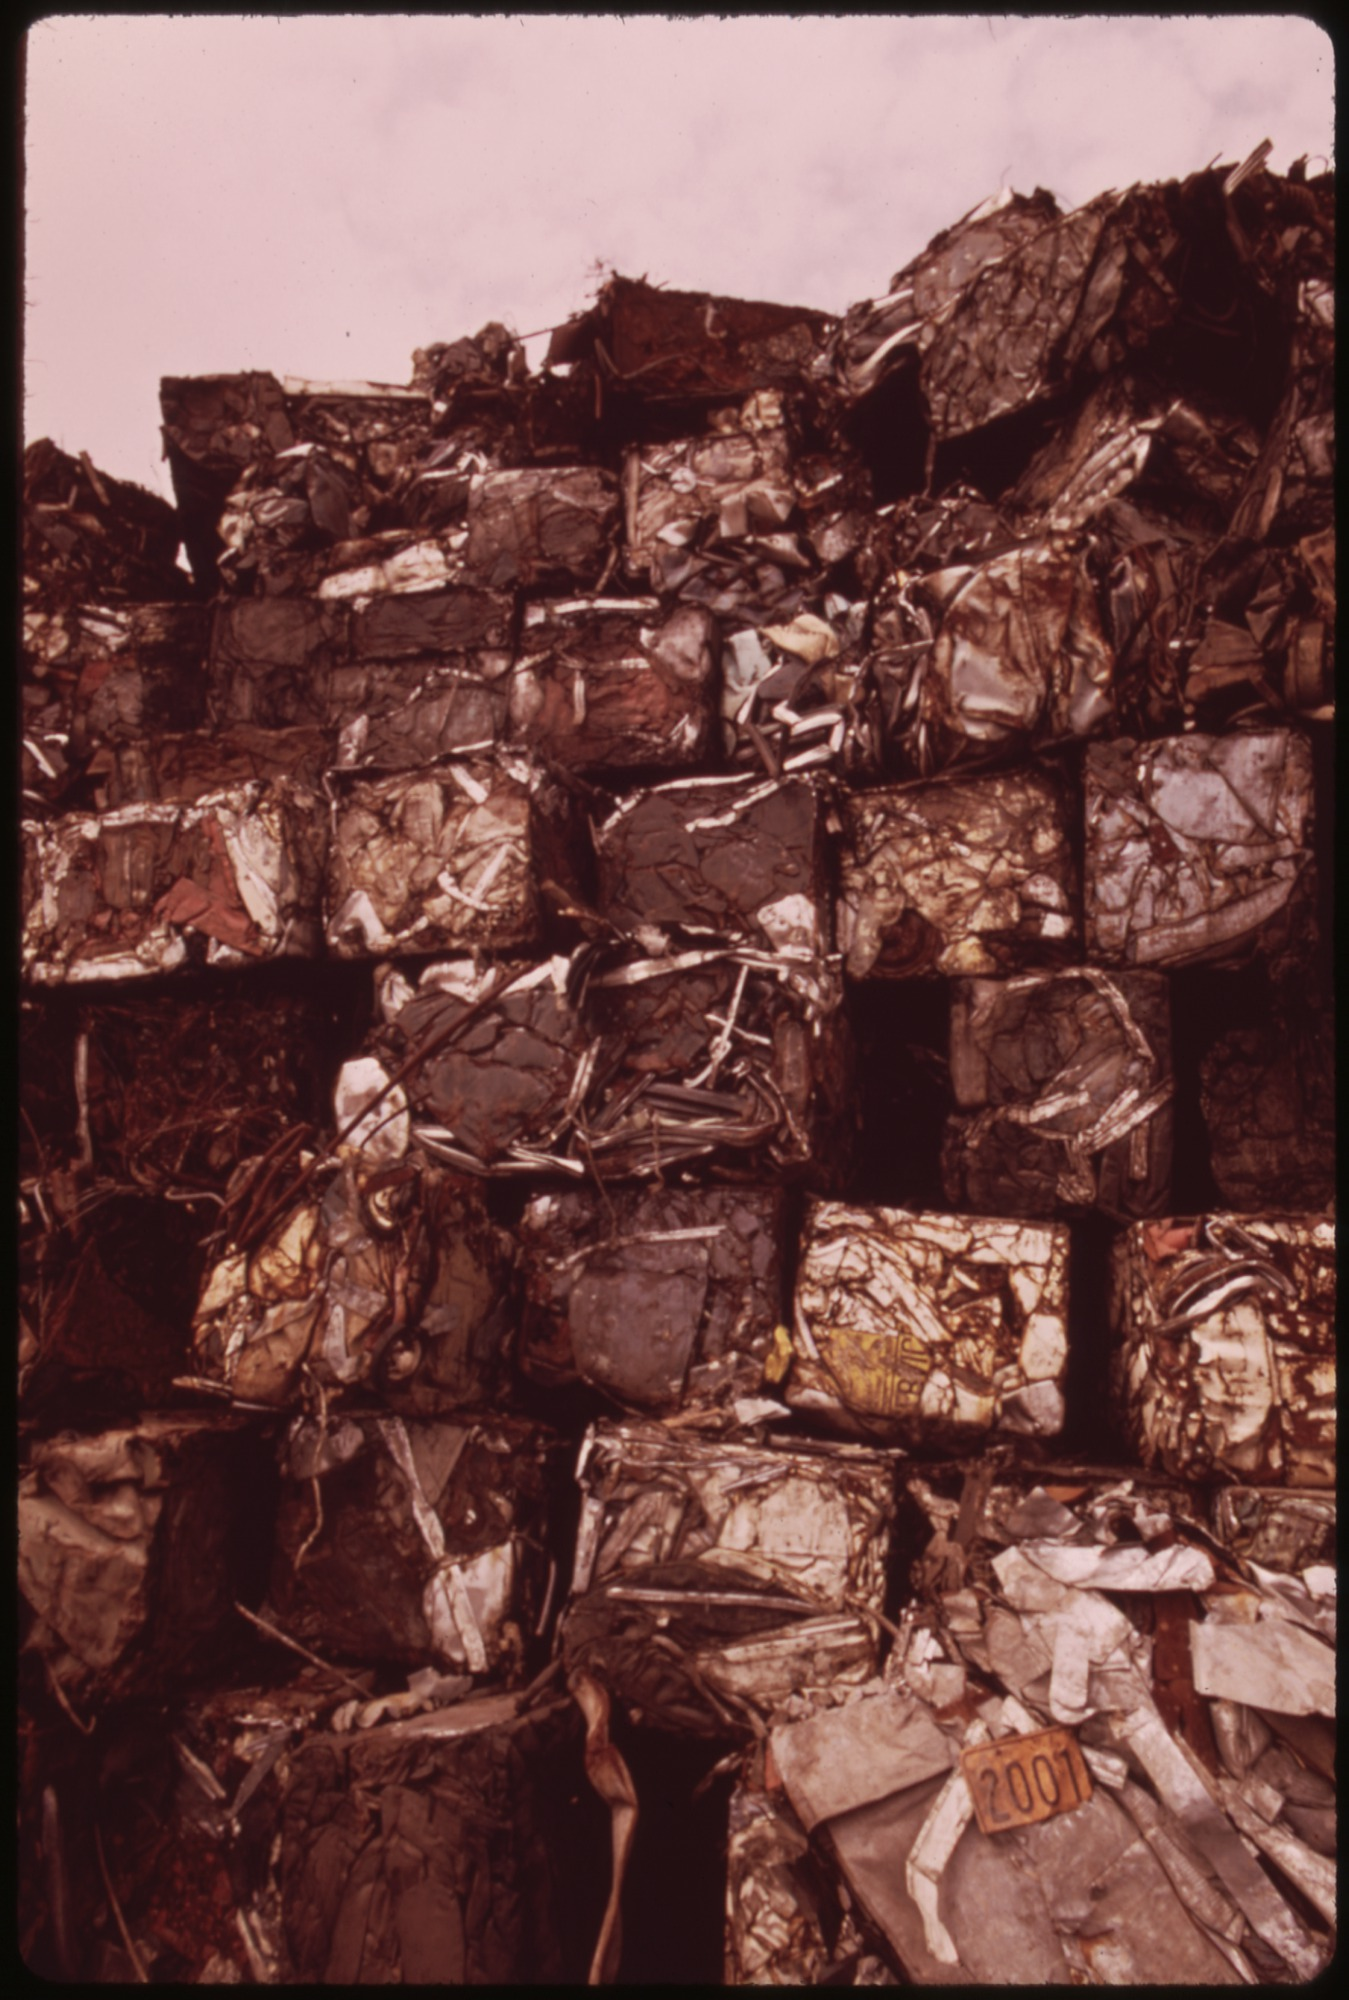
\includegraphics[width=\linewidth]{images/stack.jpg}
			
		\column{.7\linewidth}
			\begin{itemize}
				\item Kann mit \texttt{deque}, \texttt{list} und \texttt{vector} arbeiten
				\item Wichtig: \texttt{top()}, \texttt{push()} und \texttt{pop()}
				\item Laufzeit: $\mathcal{O}(1)$ für alle Einzel-Operationen
			\end{itemize}
			
			\vspace{1em}
			
			\begin{itemize}
				\item Einsatz: Bei Bedarf
			\end{itemize}
	\end{columns}
\end{frame}

\begin{frame}{\texttt{queue}}
	\begin{center}
		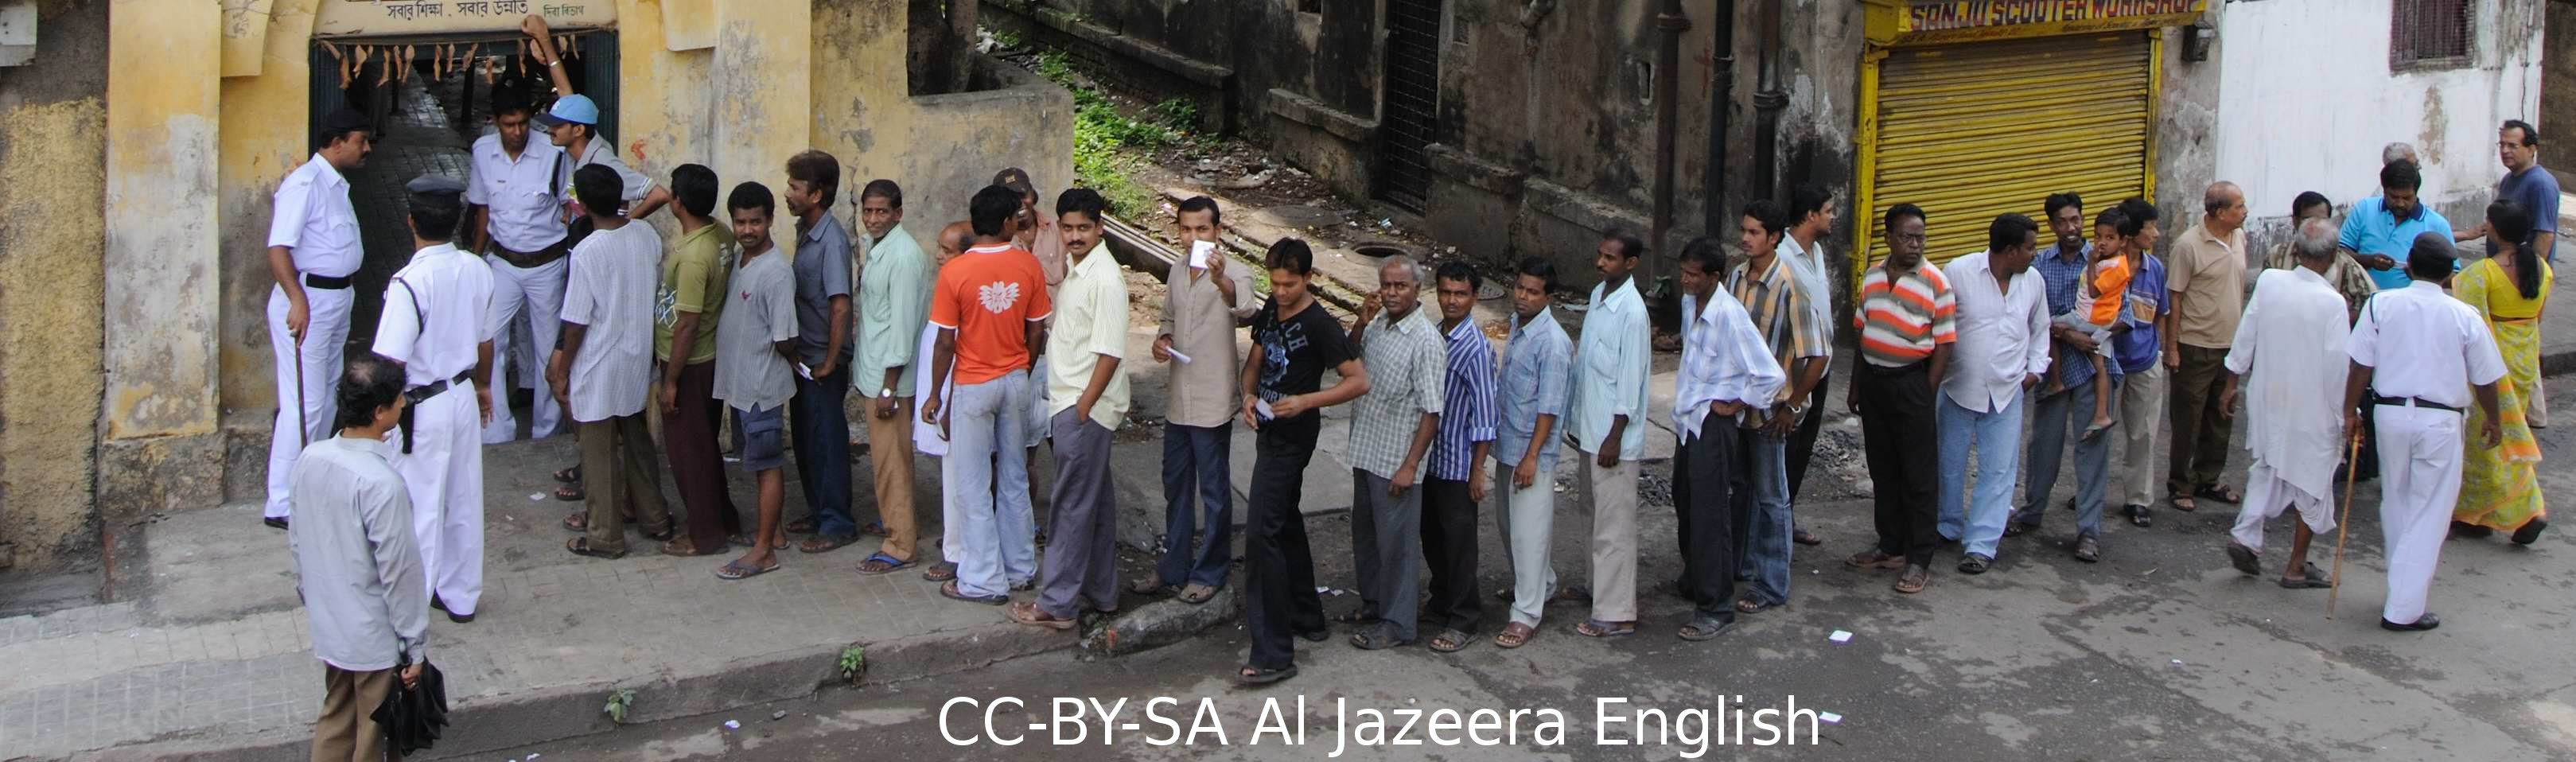
\includegraphics[width=0.7\linewidth]{images/queue.jpg}
	\end{center}
	
	\begin{itemize}
		\item Kann mit \texttt{deque} und \texttt{list} arbeiten, aber nicht mit \texttt{vector}
		\begin{itemize}
			\item \alert{Warum?}
			\pause
			\item Weil entfernen am Anfang eines \texttt{vector} \enquote{teuer} ($\mathcal{O}(n)$) ist
		\end{itemize}
		\item Wichtig: \texttt{front()}, \texttt{back()}, \texttt{push()} und \texttt{pop()}
		\item Laufzeit: $\mathcal{O}(1)$ für alle Einzel-Operationen
	\end{itemize}
	
	\begin{itemize}
		\item Einsatz: Bei Bedarf
	\end{itemize}
\end{frame}

\begin{frame}{Prioritätslisten (Priority Queues)}
	\begin{block}{Was?}
		\begin{itemize}
			\item Menge von Elementen mit einem Schlüssel
			\item Geordnet nach Schlüssel (Ordnungsrelation: $\le$)
			\item Wichtigste Operationen: 
			\begin{itemize}
				\item \texttt{insert(key, value)} 
				\item \texttt{deleteMin()} \tiny{(Alternativ: \texttt{deleteMax()}) $\rightarrow$ MinHeap/MaxHeap}
			\end{itemize}
		\end{itemize}
	\end{block}
	\pause
	\begin{block}{Wie?}
		\begin{columns}
			\column{0.7\linewidth}
				\vspace{-0.5em}
				\begin{itemize}
					\item Binäre Heaps
					\begin{itemize}
						\item Baumstruktur
						\item Jeder Knoten hat 0..2 Kindknoten
						\item Keine Löcher, Fehlstellen nur rechtsseitig in der untersten Schicht
						\item Tiefe: $\lfloor log_2(n) \rfloor$
					\end{itemize}
					\item Heap-Eigenschaft: Elternknoten $<$ Kindknoten
				\end{itemize}
			\column{0.3\linewidth}
				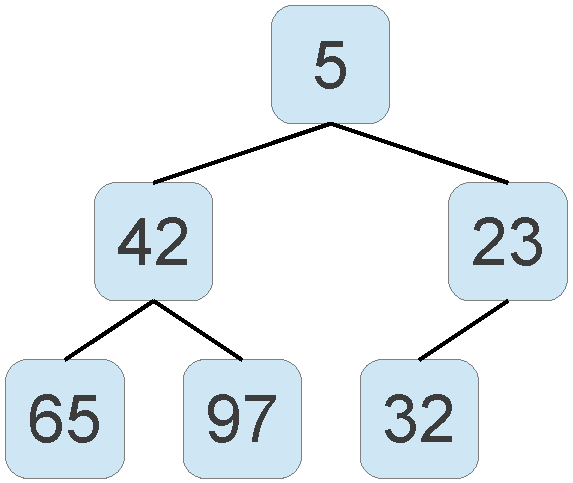
\includegraphics[width=0.95\linewidth]{images/heap.pdf}
		\end{columns}
	\end{block}
\end{frame}

\begin{frame}{Binäre Heaps: \texttt{insert()}}
	\begin{center}
		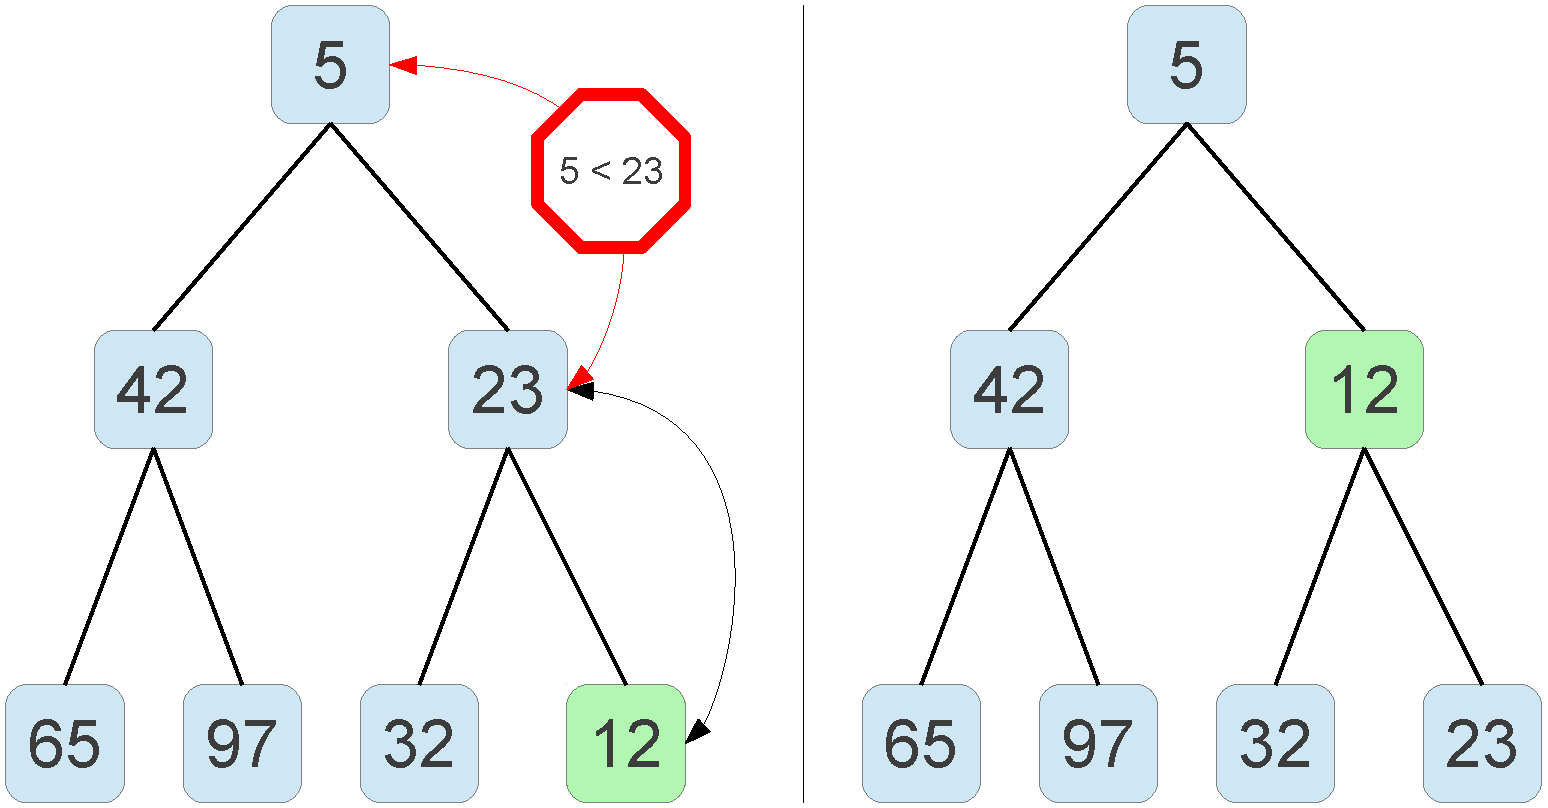
\includegraphics[width=0.90\linewidth]{images/heap_insert.pdf}
	\end{center}
\end{frame}

\begin{frame}{Binäre Heaps: \texttt{deleteMin()}}
	\begin{center}
		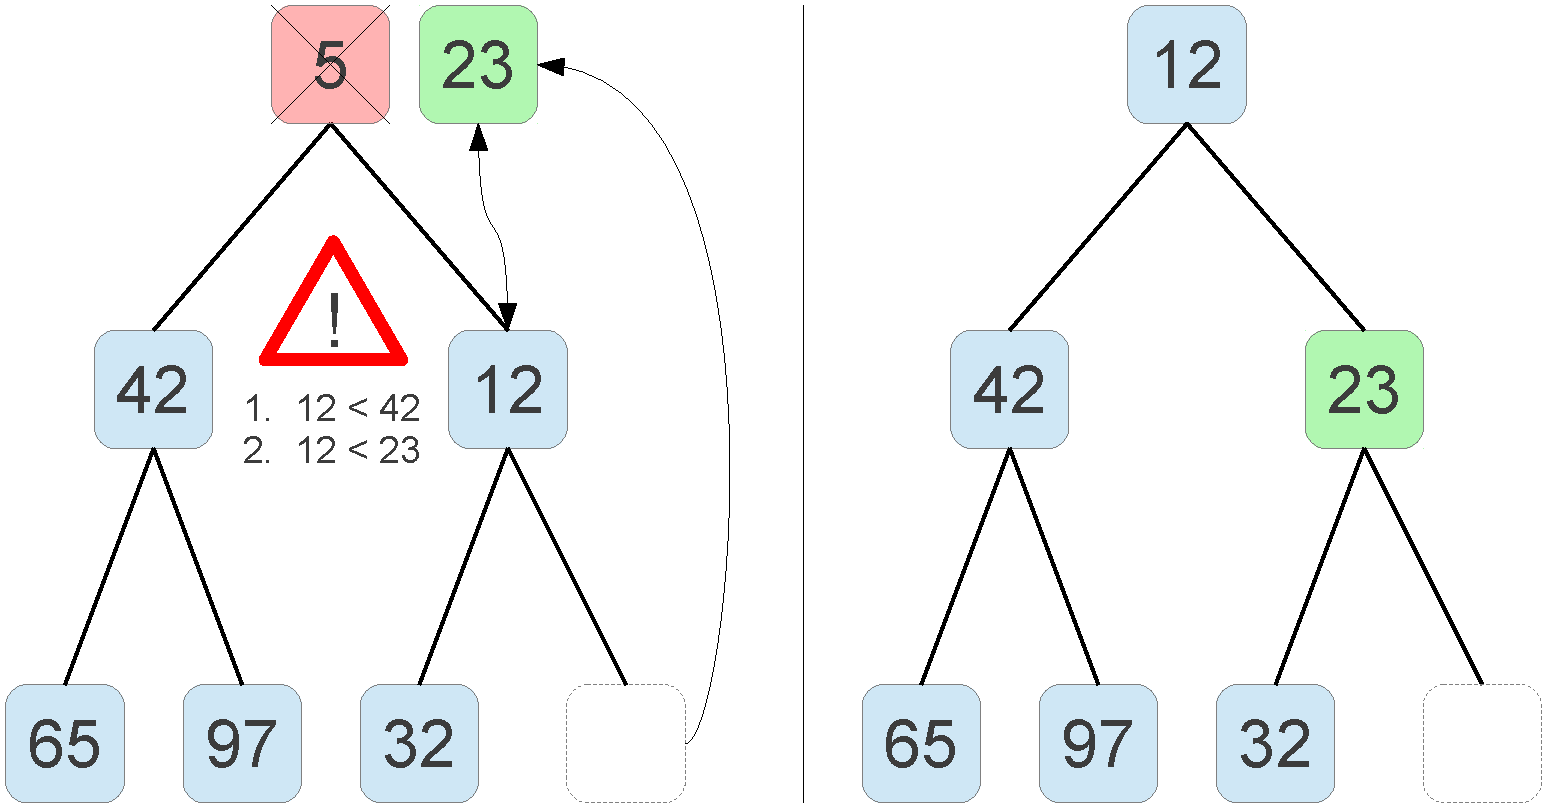
\includegraphics[width=0.90\linewidth]{images/heap_delete.pdf}
	\end{center}
\end{frame}

\begin{frame}{Binäre Heaps: Einbettung}
	\begin{center}
		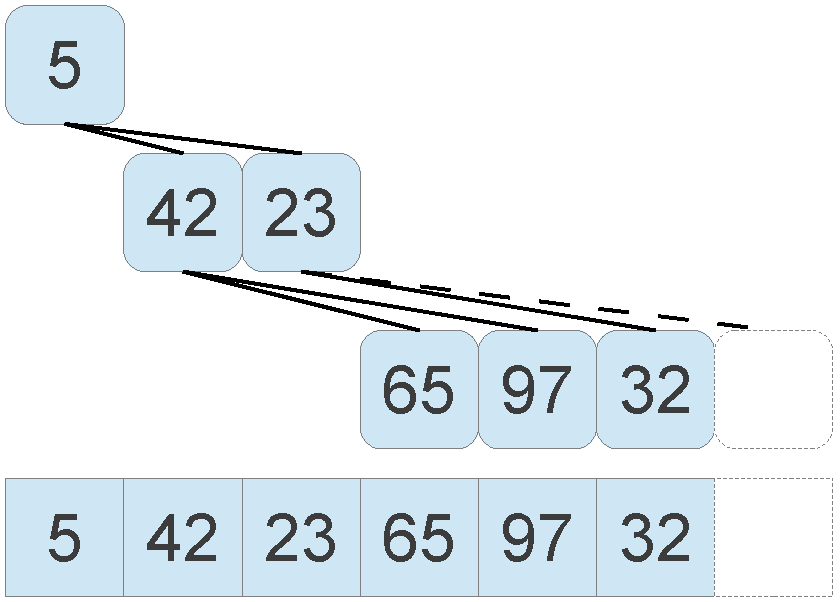
\includegraphics[width=0.85\linewidth]{images/heap_embed.pdf}
	\end{center}
\end{frame}

\begin{frame}{\texttt{priority\_queue}}
	\begin{itemize}
		\item Kann mit \texttt{deque} und \texttt{vector} arbeiten, aber nicht mit \texttt{list}
		\begin{itemize}
			\item \alert{Warum?}
			\pause
			\item Einbettung: Größere Sprünge beim Traversieren $\rightarrow$ \enquote{teuer} ($\mathcal{O}(n)$)
		\end{itemize}
		\item Wichtig: \texttt{top()}, \texttt{push()} und \texttt{pop()}
		\pause
		\item Laufzeit: $\mathcal{O}(log(n))$ für Modifikationen
		\item Heap-Eigenschaft hier: child @ parent (@ : Vergleichsoperator)
	\end{itemize}
	
	\pause
	
	\lstinputlisting[basicstyle=\scriptsize]{cpp-code/pq-usage.cpp}
\end{frame}

\subsection{associative containers}

\begin{frame}{Überblick}
	\begin{block}{Assoziative Container?!}
	 	\begin{itemize}
	 		\item Erweiterung der \texttt{priority\_queue}: Zugriff über Schlüssel
	 		\item Universell einsetzbar
	 	\end{itemize}
 	\end{block}
 	
 	\pause
 	
	\begin{itemize}
		\item \texttt{(multi)map}
		\item \texttt{(multi)set}
	\end{itemize}
\end{frame}

\begin{frame}{Sortierte Folgen}
	\begin{itemize}
		\item Zuordnung Schlüssel $\rightarrow$ Element
		\item Speicherung: Geordnet nach Schlüssel
	\end{itemize}
	\begin{center}
		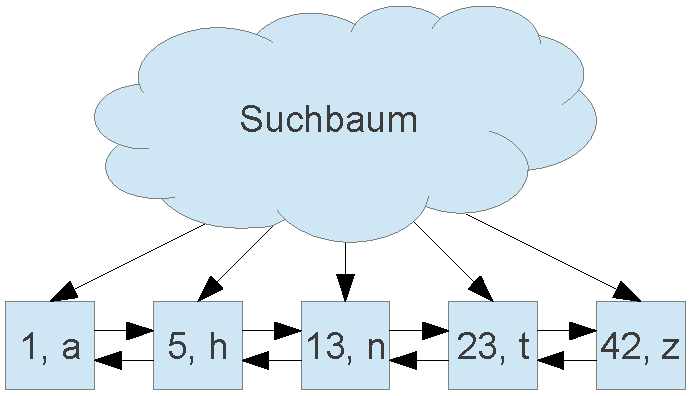
\includegraphics[width=0.7\linewidth]{images/sorted_sequence.pdf}
	\end{center}
\end{frame}

\begin{frame}{\texttt{(multi)map}}
	\begin{itemize}
		\item \texttt{multimap}: Erlaubt mehr als ein Element je Schlüsselwert
		\item Schlüssel + Element: \texttt{pair<key\_t, value\_t>}
		\pause
		\item Wichtige Operationen:
		\begin{itemize}
			\item \texttt{find(key\_t)}
			\item \texttt{operator[key\_t]}
			\item \texttt{insert(pair<\dots>)}, \texttt{erase(key\_t)}
			\item \texttt{lower\_bound(key\_t)}, \texttt{upper\_bound(key\_t)}
		\end{itemize}
		\pause
		\item Zeitkomplexität: Meist $\mathcal{O}(log(n))$
	\end{itemize}
	
	\pause
	\lstinputlisting[basicstyle=\scriptsize]{cpp-code/map-usage.cpp}
	\pause
	
	\footnotesize
	Mehr/bessere Beispiele: \url{http://www.cplusplus.com/reference/stl/map/}
\end{frame}

\begin{frame}{\texttt{(multi)set}}
	\begin{itemize}
		\item \texttt{set<type>} == \texttt{map<type, type>}
		\item[] $\rightarrow$ Element ist gleichzeitig Schlüssel
		\pause
		\item Wichtige Operationen:
		\begin{itemize}
			\item \texttt{find()}
			\item \texttt{insert()}, \texttt{erase()}
			\item \texttt{lower\_bound()}, \texttt{upper\_bound()}
		\end{itemize}
		\pause
		\item Zeitkomplexität: Meist $\mathcal{O}(log(n))$
	\end{itemize}
\end{frame}

\subsection{bitset}

\begin{frame}{\texttt{bitset}}
	\begin{itemize}
		\item Der Name ist irreführend! Besser wäre \texttt{bitvector}
		\item Kann: Bitfolgen kompakt speichern
		\item Achtung: Die Größe ist fix (Template-Parameter)
		\begin{itemize}
			\item Im Gegensatz zu \texttt{vector<bool>}
		\end{itemize}
		\pause
		\item Wichtige Operationen:
		\begin{itemize}
			\item \texttt{set()}, \texttt{reset()} und \texttt{flip()}
			\item \texttt{test()}, \texttt{any()} und \texttt{none()}
		\end{itemize}
		\item Zeitkomplexität: $\mathcal{O}(1)$
	\end{itemize}
\end{frame}

